\documentclass[letterpaper]{article}
\usepackage[margin=1in]{geometry}
\usepackage[utf8]{inputenc}
\usepackage{textcomp}
\usepackage{amssymb}
\usepackage{natbib}
\usepackage{graphicx}
\usepackage{gensymb}
\usepackage{amsthm, amsmath, mathtools}
\usepackage[dvipsnames]{xcolor}
\usepackage{enumerate}
\usepackage{mdframed}
\usepackage[most]{tcolorbox}
\usepackage{csquotes}
% https://tex.stackexchange.com/questions/13506/how-to-continue-the-framed-text-box-on-multiple-pages

\tcbuselibrary{theorems}

\newcommand{\R}{\mathbb{R}}
\newcommand{\Z}{\mathbb{Z}}
\newcommand{\N}{\mathbb{N}}
\newcommand{\Q}{\mathbb{Q}}
\newcommand{\C}{\mathbb{C}}
\newcommand{\code}[1]{\texttt{#1}}
\newcommand{\mdiamond}{$\diamondsuit$}
\newcommand{\PowerSet}{\mathcal{P}}
\newcommand{\Mod}[1]{\ (\mathrm{mod}\ #1)}
\DeclareMathOperator{\lcm}{lcm}

%\newtheorem*{theorem}{Theorem}
%\newtheorem*{definition}{Definition}
%\newtheorem*{corollary}{Corollary}
%\newtheorem*{lemma}{Lemma}
\newtheorem*{proposition}{Proposition}


\newtcbtheorem[number within=section]{theorem}{Theorem}
{colback=green!5,colframe=green!35!black,fonttitle=\bfseries}{th}

\newtcbtheorem[number within=section]{definition}{Definition}
{colback=blue!5,colframe=blue!35!black,fonttitle=\bfseries}{def}

\newtcbtheorem[number within=section]{corollary}{Corollary}
{colback=yellow!5,colframe=yellow!35!black,fonttitle=\bfseries}{cor}

\newtcbtheorem[number within=section]{lemma}{Lemma}
{colback=red!5,colframe=red!35!black,fonttitle=\bfseries}{lem}

\newtcbtheorem[number within=section]{example}{Example}
{colback=white!5,colframe=white!35!black,fonttitle=\bfseries}{def}

\newtcbtheorem[number within=section]{note}{Important Note}{
        enhanced,
        sharp corners,
        attach boxed title to top left={
            xshift=-1mm,
            yshift=-5mm,
            yshifttext=-1mm
        },
        top=1.5em,
        colback=white,
        colframe=black,
        fonttitle=\bfseries,
        boxed title style={
            sharp corners,
            size=small,
            colback=red!75!black,
            colframe=red!75!black,
        } 
    }{impnote}
\usepackage[utf8]{inputenc}
\usepackage[english]{babel}
\usepackage{fancyhdr}
\usepackage[hidelinks]{hyperref}

\pagestyle{fancy}
\fancyhf{}
\rhead{CSE 101}
\chead{Friday, March 11, 2022}
\lhead{Lecture 23}
\rfoot{\thepage}

\setlength{\parindent}{0pt}

\begin{document}

\section{Dealing with NP-Completeness}
We now talk about how to deal with NP-Completeness. First, before solving a problem, we want to see if the problem is NP-Complete. If the problem is, then we probably won't find a very good solution for it. So, at least, you have an excuse for not having a better algorithm. However, if you need to solve the problem, well, you still need to find some way to solve it. In this section, we'll briefly talk about ways to solve such problems. 

\bigskip 

Consider the following statement: \emph{if your problem is NP-Hard/NP-Complete, then unless $P = NP$, there is no algorithm that gives the exact answer to your problem on all instances in polynomial time.} Despite not being able to get around the fact that you might not be able to solve such problems efficiently, there are loopholes in this statement that can be exploted.
\begin{itemize}
    \item ``\textbf{all instances}'': there are worst-case instances which can be very hard to solve. But, the instances that you're working on is easier. For example, maximum independent set is a hard problem, but maximum independent set of trees is not. So, see if you can make further assumptions. 
    \item ``\textbf{exact answer}'': you sometimes do not need the \emph{best} answer. It's okay to have a good answer. This leads to the notion of approximation algorithms. 
    \item ``\textbf{polynomial time}'': for finite input sizes, or smaller input sizes, the runtime of your algorithm might not matter. So, an \emph{efficient brute-force} algorithm might be good enough. 
    \item ``\textbf{P = NP}'': If you can prove that $P = NP$, then you can solve whatever problems you would like in $NP$. 
\end{itemize}

\subsection{Sudoku}
Consider the logic puzzle Sudoku, where you have a $9 \times 9$ grid of numbers with 1 - 9 so that:
\begin{itemize}
    \item Each row has all numbers. 
    \item Each column has all numbers. 
    \item Each of the main $3 \times 3$ sub-squares has all numbers. 
    \item Some entries are pre-filled. 
\end{itemize}
For a fixed board size, you can't really say that this problem is in NP. However, there is an obvious generalization which is formally a NP-Hard problem. 

\subsubsection{Brute-Force}
Generally speaking, you cannot do much better than brute-force saerch. However, we note that, even for a fixed board size of $9 \times 9$, a brute-force search would consider $9^{81}$ possibilities. This would essentially take longer than the lifespan of the universe. However, people can solve them while waiting for something. How is this the case? 

\subsubsection{Deductions}
One way to make progress is to make deducations. In particular: 
\begin{itemize}
    \item We can use the rules to show that some square can only be filled out in one way. 
    \item We can use that information to help fill out more squares. 
    \item If you're lucky, you can keep going until the entire problem is solved. 
\end{itemize}
To see an example of how this would work, consider the 3-SAT problem $x \land (\overline{x} \lor y) \land (\overline{x} \lor \overline{y} \lor z)$. 
\begin{itemize}
    \item For the whole statement to be true, each clause must be true. So, $x = \text{True}$.
    \item If we simplify this, we now get $y \land (\overline{y} \lor z)$. Therefore, $y = \text{True}$. 
    \item Simplifying this further gives us $z$. Therefore, $z = \text{True}$. 
\end{itemize}
So, instead of having to check every possible options, we can just make a sequence of logical deductions which led us to the answer. 

\subsubsection{Getting Stuck}
If we just have simple rules like this, we'll get stuck pretty quickly. This especially applies if you have harder problems. So, how do you get unstuck? 
\begin{itemize}
    \item Use stronger deduction rules. In the case of Sudoku:
    \begin{itemize}
        \item Find a square that only one number can fill.
        \item Find a region with only one place for a given number to be put. 
        \item Find a pair of squares in the same row that must contain two numbers (which then cannot appear elsewhere in that row).
        \item Find a rectangle whose corners must contain 2 copies of a number. That number cannot appear elsewhere in those rows/columns.
        \item Find 3 rows and 3 columns whose intersections must contain 3 copies of a number. That number cannot appear elsewhere in those rows and columns.
    \end{itemize}
    This helps cuts down a bunch of possibilities which can simplify your search space. 

    \item Guess and check. For example, you can make a guess, and then use the deduction rules to see if you can reach a contradiction. If you reach a contradiction, then you know that the guess you made is wrong so you can guess again. Formally, this is known as \emph{backtracking}.
\end{itemize}

\subsection{Finding Exact Solutions to NP-Complete/Hard Problems}
There are two strategies to find exact solutions. 

\subsubsection{Backtracking}
The idea behind backtracking is as follows. 
\begin{verbatim}
    Search(Problem P, Search Space S):
        If you can find a contradiction:
            return 'no solution' 
        Split S into subproblems S1, S2, ... 
        For each i: 
            Run Backtracking(P, Si)
        Return any solutions found. 
\end{verbatim}
Essentially, the idea is to try every possible solution in $S$. However, if we can reach a contradiction -- especially early on -- then we can cut our search space by a significant factor. 

\bigskip 

Another thing to consider is how you split your search space. Generally, you want to branch on variables that have a lot of deductive power -- essentially, variables which may lead to a contradiction very early on. 

\bigskip 

Note that backtracking works well for decision problems. However, for optimization problems, not so much. So, we introduce the idea of \emph{branch and bound}.

\subsubsection{Branch and Bound}
For optimization problems, we need to keep track of the best solutions so far. Then, instead of a contradiction, what you need to do is \emph{bound} the best solution in $S$ (the space you're searching over). Then, if it's \emph{worse} than the best so far, then stop. 

\bigskip 

Essentially, the idea is as follows. 
\begin{verbatim}
    BranchAndBound(Best, Search Space S):
        If UpperBound(S) <= Best:
            Return 'no improvement' 
        If S is a full solution: 
            Return value of S 
        Split S into subproblems S1, S2, ... 
        For each i: 
            New = BranchAndBound(Best, Si)
            Best = Max(New, Best)
        Return Best 
\end{verbatim}


\subsection{Heuristic Search}
Heuristic search is this idea where we relax one of the rules to find an answer. For example, we can relax the rule that we want the exact answer. Often times, especially for optimization problems, we don't necessarily need the best answer; we only need a ``good enough'' answer. 

\subsubsection{Hill-Climbing}
The high-level idea is what is known as \emph{hill-climbing}. The idea is that we find $x$, and then we try all $y$ near $x$. If $f(y) > f(x)$, then we set $x$ to be $y$. This idea would be repeated until you don't really see an improvement. 

\subsubsection{Getting Stuck}
An issue is that you can get stuck, though. For example, suppose you're at the bottom of a hill. There are going to be a lot of local maximum points, which your algorithm might interpret as the maximum. However, we note that there could very well be an absolute maximum point that the algorithm can't find. 

\subsubsection{Getting Unstuck}
There are several ways to get unstuck. 
\begin{itemize}
    \item Randomized Restart: If you try many starting points, you might be able to find the one that is the true maximum. In the hill-climbing analogy, this just means starting at different points in the hill. 
    \item Expand Search Area: Instead of looking for changes in a small, restricted area, you could expand how far you saerch to hopefully find a better answer. The disadvantage of this is that the larger areas could take more work. However, at least it's harder to get stuck. In the hill-climbing analogy, this means that, rather than taking one step to see if you can find a higher point, you could take multiple steps around. 
    \item Simulated Annealing: At the start of the algorithm, you can take big, random steps. This will hopefully get you to the right hill. Then, as the algorithm progresses, the step distance decreases and the algorithm starts to fine-tune more precisely. This works well, in practice, for a number of problems. 
\end{itemize}
In either case, it's still no guarantee of finding the actual maximum in polynomial time. 


\subsection{Approximation Algorithms}
An $\alpha$-approximation algorithm is an algorithm that always obtains the optimal value up to a factor of $\alpha$. 

\bigskip 

For example, a 2-approximation algorithm is an algorithm that obtains the optimal value up to a factor of 2; if you're maximizing, you're at least a half of the maximum value, and if you're minimizing, you're at most twice of the optimal value. 

\bigskip 

An approximation answer doesn't necessarily give you the best answer, but at least it gives you some rigorously proven guarantees about how good your answer is. 


\subsubsection{Problem: Vertex Cover}
Given a graph $G$, find a set $S$ of vertices so that every edge of $G$ contains a vertex of $S$ and so that $|S|$ is as small as possible. 

\bigskip 

For example, consider the graph below.
\begin{center}
    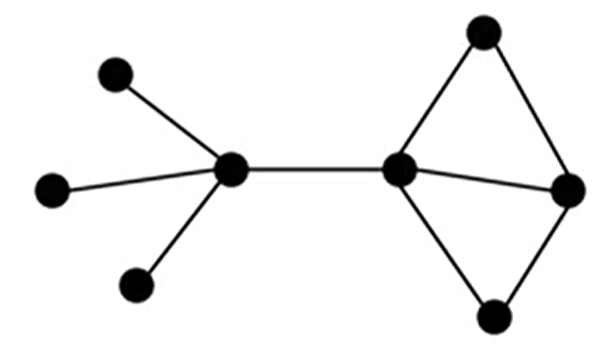
\includegraphics[scale=0.5]{../assets/vertex_cov.png}
\end{center}
The minimal size is 3, and is given by: 
\begin{center}
    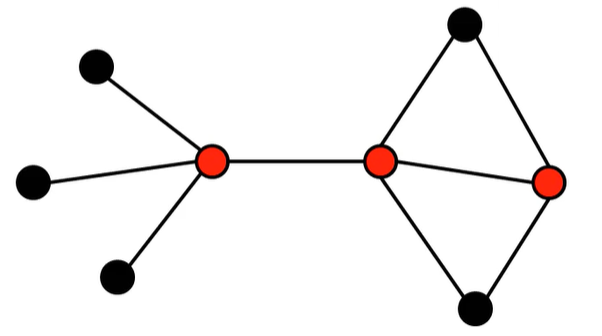
\includegraphics[scale=0.5]{../assets/vertex_cov_2.png}
\end{center}

\subsubsection{Greedy Algorithm for Vertex Cover}
The greedy algorithm for the vertex cover problem is as follows: 
\begin{verbatim}
    GreedyVertexCover(G):
        S = {}
        While S doesn't cover G:
            (u, v) = some uncovered edge 
            Add u and v to S
        Return S
\end{verbatim}
We note that this is a 2-approximation algorithm. 

\subsubsection{Example of Algorithm on Graph}
In the graph above, we note that this algorithm could potentially find the following vertices:
\begin{center}
    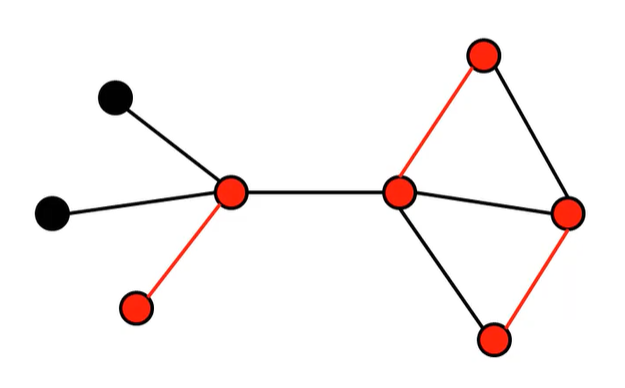
\includegraphics[scale=0.5]{../assets/vertex_cov_3.png}
\end{center}
The algorithm finds $k$ edges and returns $2k$ vertices. These edges are vertex-disjoint, i.e. no two edges could share a vertex since we added both vertices whenever we account for an edge. So, any cover must have at least one vertex on each of these edges. So, the optimal cover has size at least $k$, but we have one of $2k$. 


\end{document}